%----------------------------------------------------------------------------------------
%	PACKAGES AND DOCUMENT CONFIGURATIONS
%----------------------------------------------------------------------------------------

\documentclass{article}

\usepackage[version=3]{mhchem} % Package for chemical equation typesetting
\usepackage{siunitx} % Provides the \SI{}{} and \si{} command for typesetting SI units
\usepackage{graphicx} % Required for the inclusion of images
\usepackage{natbib} % Required to change bibliography style to APA
\usepackage{amsmath} % Required for some math elements 
\usepackage{enumitem}% For lists
\usepackage{mathptmx}% For textbf
\usepackage{float} %for correct image placement
\usepackage{textcomp} % for texttildelow
\usepackage[T1]{fontenc} % allows use of less than <
\usepackage{booktabs} % for tables


\setlength\parindent{0pt} % Removes all indentation from paragraphs

\renewcommand{\labelenumi}{\alph{enumi}.} % Make numbering in the enumerate environment by letter rather than number (e.g. section 6)

%\usepackage{times} % Uncomment to use the Times New Roman font

%----------------------------------------------------------------------------------------
%	DOCUMENT INFORMATION
%----------------------------------------------------------------------------------------

\title{M152A - Lab 4 \\ Design Lab \\ The Multiplayer Tank Experience} % Title

\author{Markus \textsc{Notti} - 904269231 \\ Kyle \textsc{Baker}  - 604273748 \\ Niels \textsc{Pineda} - 604272353} % Author name


\date{\today} % Date for the report

\begin{document}

\maketitle % Insert the title, author and date

%----------------------------------------------------------------------------------------
%	SECTION 1
%----------------------------------------------------------------------------------------

\section*{Introduction}

%Summarize background information
%about the lab and the detailed design requirements. It?s very important to
%make sure you are designing the right thing before starting.

In this lab, we implemented a basic multiplayer tank game utilizing the VGA for the main display, buttons and switches on the board for controls, and the seven segment display for additional in game information display.

Our game was played in the following manner:
Each of the two players playing the game controls a tank and fires projectiles at his opponent from the opposite side of the map, displayed on the VGA.  To fire, the player 1 and player 2 would press the \textit{fire1} and \textit{fire2} buttons respectively. As the players fire the projectiles using the buttons on the FPGA board, the players are also able to adjust the initial velocity and angle of the projectiles using additional buttons.  How long the \textit{fire1} and \textit{fire2} buttons are held down by the players determines the projectiles' initial velocity, and the angle can be adjusted by clicking either the \textit{angleUp} button to raise the angle or the \textit{angleDown} button to lower the angle. 
\\
\\
If a player's tank is struck by a hostile projectile, the player's tank loses health, which is immediately updated on the 7-segment display. If the projectile makes a direct hit upon the tank, the player's health is reduced by 14HP. If it is only a glancing blow the player's health is reduced by only 7HP.  The health display for both of the players' healths was also configured to display the player's own health facing the correct player. In other words, since the players themselves must be on opposite sides of the board to play the game, each player can see his own health, because it is flipped to the perspective of the player who's health it is displaying. 

If a tank reaches a health of 0HP, that tank turns red marking the end of the game and victory for the player controlling the other tank.  The game can then be reset by flipping the \textit{rst} switch on the board.
\\
\\
Behind the scenes, a clock module, which along with the other modules, will be discussed in more detail later, created three separate clocks which would drive the program.  The three clocks created were 25MHz, 500Hz, and 50Hz.  The 25MHz clock was responsible for driving the VGA controller, the 500Hz clock drove the seven segment display, and the 50Hz clock was responsible for updating the position of the tanks and the projectiles on screen. 
\\

In order for all of this gameplay to be a reality, we needed to design and implement the following set of features:
%TODO: pdf/screenshot of the features list (as edited by matt millar himself)
 
%----------------------------------------------------------------------------------------
%	SECTION 2
%----------------------------------------------------------------------------------------

\section*{Design Description}

%Design description (15%). Document the design aspects including the basic
%description of the design, modular architecture, interactions among the
%modules, and interface of each major module. You should include schematics
%for the system architecture. You can also include figures for state machines
%and Verilog code when needed.

% TODO: Make circuit diagram
% TODO: Make sure the figures referenced are correct

When designing the lab, we created 8 main modules \textit{clock}, \textit{vga}, \textit{sevenSeg}, \textit{tankL}, \textit{tankR}, \textit{projL}, \textit{projR} and \textit{collisionDetector} all running in the main module \textit{game}.  The clock module created 3 slower clocks to regulate other parts of the program, while the rest of the modules, their names relatively self explanatory, contained the program's logic.

\subsection*{Clock Module - \textit{clock}}

The clock module took as input a 100MHz clock and outputted three separate clocks to govern the rest of the program: a 25MHz clock, a 500Hz clock, and a 50Hz clock.  This was implemented by 3 simple counters. The 25MHz counter would count to 4, the 500Hz clock would count to 200,000, and the 50Hz clock would run to 2,000,000.  At the posedge of the 100MHz clock, the counts would increment until they reached their respective maximums, triggering the appropriate output clocks to 1. After reaching this maximum value, the counters would drop back to zero and start their counts over again.  This clock module was the beating heart of our software, controlling the rates at which all logic would be calculated, all input would be read and all output would be written.

\subsection*{VGA Module - \textit{vga}}

Our VGA module was essentially a controller we designed to handle the VGA functionality for the program.  This was probably the most complicated of the lab for us, because it took a lot of trial and error to get it working.  Our VGA controller module takes as the 25MHz clock created by the clock module and produces as output 8 wires which make up the color composition of the pixel to be drawn and two wires \textit{Hsync} and \textit{Vsync} to govern the VGA.  \\
\\
In order to implement this controller, two counters, \textit{counterX} and \textit{counterY}, tracked the location of the VGA sweep as it swept across the screen and down the screen.  In addition to tracking the location of the VGA sweep on the 640x480 display to figure out when to draw what pixels, the counters were responsible for tracking when exactly it was even appropriate to begin outputting values to the 8 wires governing the pixel color. The tricky part about designing the VGA controller was this specific timing.  As illustrated further by the image below, there are very specific periods of time where no color combination must be output, and there are specific times when the \textit{Hsync} and \textit{Vsync} must be fired to indicate that a new section of the display is about to be drawn.  For every line, there would be a front porch for 8 cycles, a horizontal sync period where Hsync would be fired for 96 cycles, a back porch for 40 cycles, an 8 cycle left border, then a 480 cycle display followed by an 8 cycle right border.  For the periods mentioned above, the colors outputted by the vga module to the VGA were all set to 0.  \textit{counterX} tracked how many cycles had passed to give the program working knowledge of what period it was in. During the display period is where the appropriate objects were drawn to screen.  The Vertical Sync had similar periods with slightly different cycle count.  The exact count is displayed below in the image.  Note that where the image says 'pixels', we implemented our controller so that each cycle moved onto the next pixel, so in this situation, pixels can be considered equivalent to cycles.

\begin{figure}[H]
	\begin{center}
		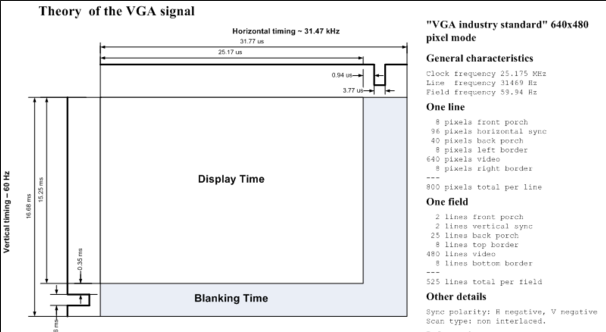
\includegraphics[width=1\textwidth]{vgaTheory} 
		\caption{Basic VGA theory upon which we based our VGA controller}
	\end{center}
\end{figure}

\subsection*{Seven Segment Display Module - \textit{sevenSeg}}

This module was the controller we designed to handle the seven segment display.  It would be passed both of the players' healths and it would display player 1's health facing him, and player 2's health facing opposite, so each of the players can look down at the seven segment display from his respective side of the board and see how much health he has remaining. \\
\\
The encoding of the tank health into a form readable and displayable by the seven segment display was done using two priority encoders, one for the digits that faced player 1, and one for the digits that faced player 2.  Once the digits were all encoded by the priority encoders, the 4 digits were  separately displayed at a frequency of 500Hz, governed by a clock that was passed into the module as input after being created by the clock module.  By displaying only one digit at a time, and displaying a different digit 500 times a second, it seems to the human eye that all four digits are being displayed simultaneously.

\subsection*{Tank Module - \textit{tankL}, \textit{tankR}}

The tank module was designed with the purpose of controlling the location and the movement of both players' tanks on screen.  While it didn't make them actively move across the screen, the job of the VGA controller, the tank module looked for movement button presses from the players and updated the tanks' positions accordingly, outputting them to the projectile modules so they knew where to place the projectiles on screen upon initially firing, and to the VGA module so that the VGA knew where to draw them.  
\\
\\
Not only did the tank module handle listening for movement buttons \textit{btnL} and \textit{btnR} in order to update the position of the tanks accordingly, it also listened for \textit{angleUp} and \textit{angleDown} buttons to adjust the angles at which the projectiles would be firing from the tanks.  Every time either the angle up or angle down buttons would be pressed, the tank module would add or subtract 5 degrees from the angle of the relevant tank.  This angle value would then be passed into the projectile module.
\\
\\
It should also be noted that due to some minor issues we had when we created two instances of the tank module, one for player 1 and one for player 2, we decided to do a quick work around and make them two separate modules.  Since they are effectively the same, I have considered them the same for the sake of this report.

\subsection*{Projectile Module - \textit{projL}, \textit{projR}}

The projectile module contained all of the logic required to simulate the motion of the projectile as if its been fired from the barrel of a cannon.  This module takes as input the tank's location and the angle at which that tank is currently set to fire its projectile.  The projectile module then takes the angle and uses a priority encoder to retrieve the correct initial x and y velocities at which it should be fired.  Then, if the appropriate fired button is pressed, the projectile takes the initial position of the appropriate tank and is assigned the initial velocities found by the priority encoder.  Next, the new position of the projectile is determined 50 times a second, and is outputted to vga to be displayed.  In order to keep the projectiles flight from being adversely affected by the movement of the tank while the projectile is in flight, updates to the tank's initial position and angle are stopped while the projectile is in flight. Once the projectile hits its target or falls off the screen, the projectile module begins again to listen.
\\
\\
Like the tank module mentioned above, the same problem was occurring for us, so we went ahead and made two separate projectile modules, as it solved our problem.  However, in the same way, I have considered them two instances of the same module for the sake of simplicity in explanation.

\subsection*{Collision Detector Module - \textit{collisionDetector} }

The collision detector module, as the name suggests, was responsible for monitoring the positions of the tank modules and the projectile modules and listening for any overlap.  It was also responsible for relaying that information to the rest of the program. It simply would take in as input all of the positions of the objects mentioned above and check for overlap.  If there was overlap, it would simply set a t1\_col flag to 1 or a t2\_col flag to 1 depending on which tank was hit.  The projectile module would pick up this flag and reset, and the seven segment controller module would also pick up this flag and update the health of the tanks on the display accordingly.

\subsection*{Digital Logic Design}

\begin{figure}[H]
	\begin{center}
		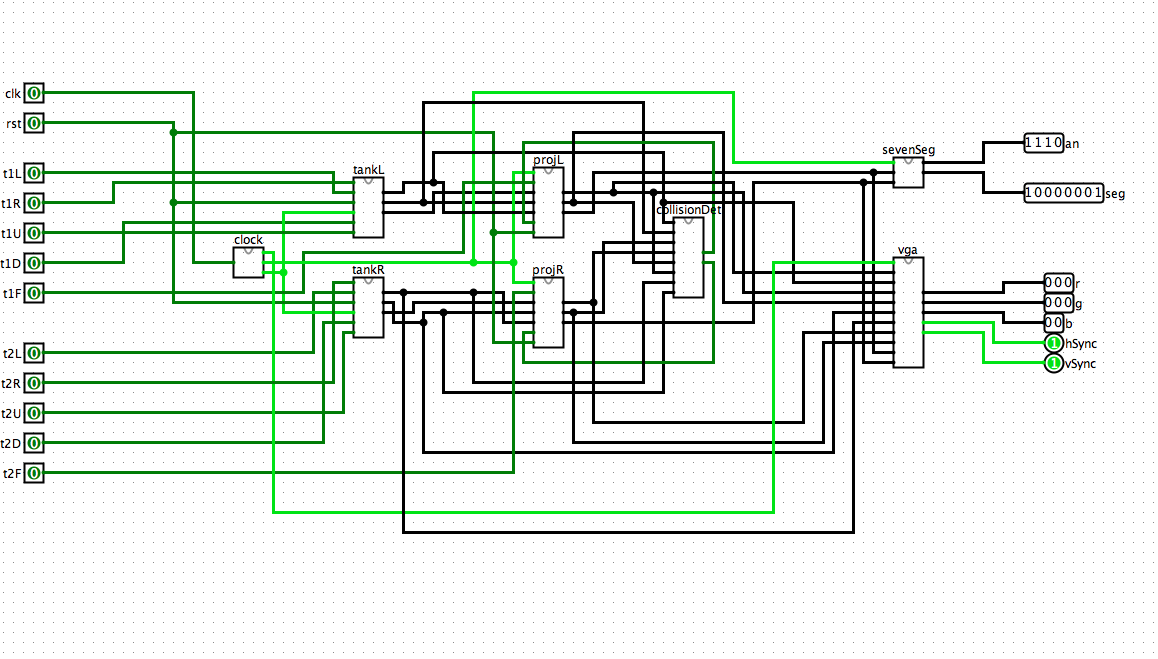
\includegraphics[width=1\textwidth]{game.png} 
		\caption{Game module logic}
	\end{center}
\end{figure}

The above image shows the top game module we had. It was broken down into seven distinct modules: a clock, tankLeft, tankRight, projectileLeft, projectileRight, collisionDetector, sevenSeg, and vga. Each of these modules will be described in detail below. The game module takes in 12 inputs. These inputs are a clock, a switch representing a game reset, and 5 buttons for each player (left, right, angle up, angle down, and fire). The clock module takes in a 100 MHz clock and outputs three seperate clocks, one to be used in the tank and projectile modules (slowest), one for the collision detector and seven segment display modules (next fastest), and the fastest clock for the vga module. The tank modules outputs the location of the tanks to three places: the vga module, the projectile module, and the collision detection module. It also outputs its angle to the projectile module. The projectile motion module takes in the fire button as input and the location of the tank. It also takes in output from the collision detection module to tell when the projectile has hit a tank. When a projectile is fired, it starts its motion. It will then output its location to the vga and collision detection modules. The projectile module also keeps track of tank health, which is outputted to the vga and seven segment display modules. The seven segment display module takes in tank healths as input and outputs to the seven segment display on the board. The vga module takes in tank and projectile location information to display the objects on screen as output. It will also take in tank health from the projectile modules.


\begin{figure}[H]
	\begin{center}
		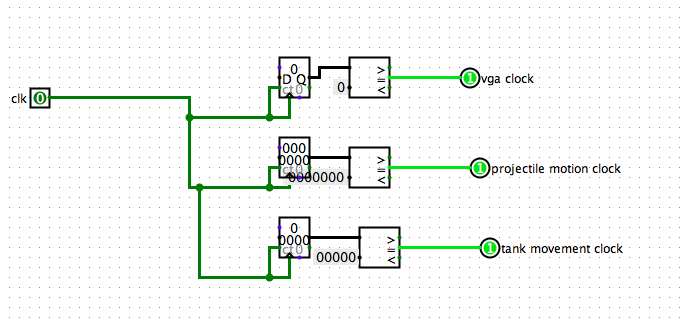
\includegraphics[width=1\textwidth]{clock.png} 
		\caption{Clock module logic}
	\end{center}
\end{figure}

Our clock module takes in a 100 MHz clock and uses that to output three seperate clocks. We used counters that overflow to simulate the different speed clocks. When the counters overflow (i.e. they equal zero), we output a high signal for the clock.

\begin{figure}[H]
	\begin{center}
		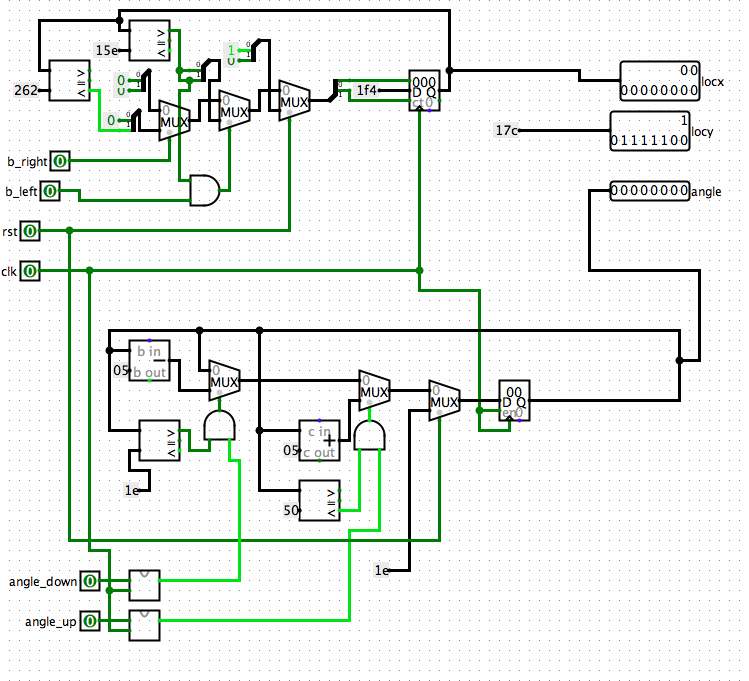
\includegraphics[width=1\textwidth]{tank.png} 
		\caption{Tank module logic}
	\end{center}
\end{figure}

The tank takes in inputs from 4 buttons, angleUp, angleDown, moveLeft, moveRight. It also takes in a clock and a reset signal. To calculate the tank's x location, We used a counter. This register was incremented when the moveRight signal was high (increase x value), and decremented when the moveLeft signal was high (decrease x value). Comparators are used to make sure the tank never moves past a certian threshold (off the screen or on the other tank's side of the screen). The same basic thinking applies to the design of the angle calculator. A counter was used, with comparators used to make sure the angle never passed its minimum or maximum values. Muxes are used to simulate if, else if, else statements here. The tank's y location is kept constant as the tank itself can't ever move up or down. In our implementation, we had two seperate tank modules. The only differences were the constants used to determine tank movement boundaries and initial starting location.

\begin{figure}[H]
	\begin{center}
		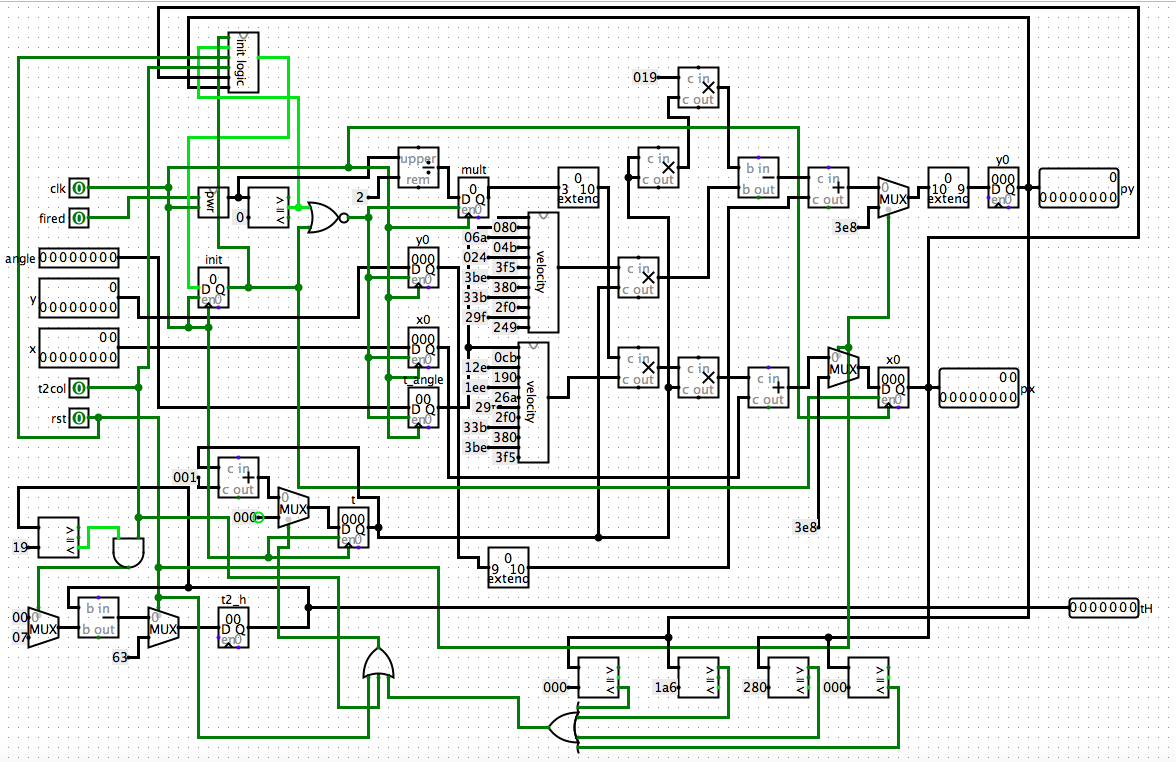
\includegraphics[width=1\textwidth]{projectile.png} 
		\caption{Projectile module logic}
	\end{center}
\end{figure}

The projectile module takes in the tank's x and y location, the angle the tank is pointing at, the fired bit, a colision bit, the reset flag, and a clock. It outputs it's x and y location and the opposing tank's health. This digital logic implementation makes use of three black box modules, the velocity module, the init logic module, and the power module which are described below. The power module both acts as a debouncer and as a power gague for the stregth of the shot. It'll output a three bit wire, representing how strong the shot is. We have a register named init. This register helps determine when to update a projectile's location. It basically keeps track of when a projectile has already been fired. If a projectile has not been fired, but the output from the power module is not zero (the fire button has been pressed), we want to update the x0, y0, and angle values that will be used in projectile motion equations to be those that are input from the tank module. The logic updating the init value was given it's own module. When the projectile fires, we change init to be 1. While init is 1, we don't update the x0, y0, or angle registers, because those should be constant throughout the projectile's motion, despite where the tank moves. The angles are passed into the velocity module, which essentially use a series of MUXes to decide what the base x and y velocities of the projectile should be. The adders, multipliers, and subtracters are used to calculate the projectile motion equations, which eventually become output. If the projectile is off screen or if it collides with a tank, the projectile location is set just off screen so it is not displayed by the vga module. This module also keeps track of the opposing tank's health. The logic for this is shown at the bottom of the figure with the t2h register. A MUX leads into this register. This MUX will make the register's value get reset back to 99 when the reset flag is true. Otherwise, on a colision, t2h's value is passed to a subtractor to decrement the value by seven. A comparator is used to make sure the health value never dips below 0. In out implementation, we had two seperate modules, the only difference being that one had negative x velocity (the right tank's projectile).

\begin{figure}[H]
	\begin{center}
		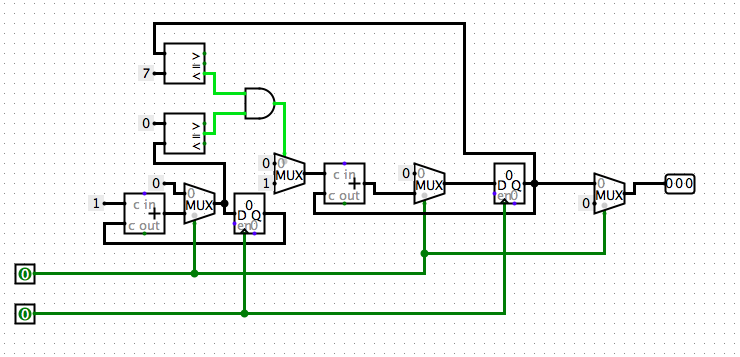
\includegraphics[width=1\textwidth]{power.png} 
		\caption{Power module logic}
	\end{center}
\end{figure}

This module calculates a multiplier that represents how fast the projectile will be shot. It basically is a modified debouncer. When a counter overflows, another counter is incremented. When the button is released and is at a low signal, whatever value is in the second counter is outputted. The second counter is updated by an adder. The input to this adder is the value of the register itself and either a 1 or a 0. If the value of the first counter overflowed and is now a 0, and the value of the second counter is less than 7 (the max multiplier), we add 1. Otherwise, we add 0, thereby keeping the value constant. When the button signal is low, all regesters are reset to 0. 

\begin{figure}[H]
	\begin{center}
		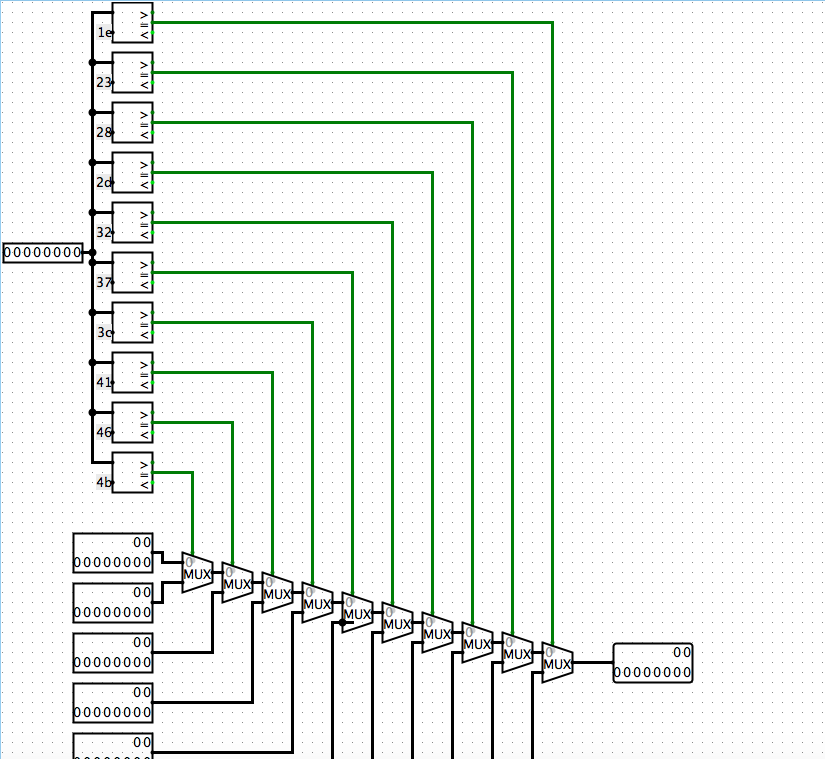
\includegraphics[width=1\textwidth]{prienc.png} 
		\caption{Velocity module logic}
	\end{center}
\end{figure}

This module basically uses a series of comparators and MUXes to make a huge switch statement. This is used to find what a velocity should be, given an angle input and input of a list of possible velocities.

\begin{figure}[H]
	\begin{center}
		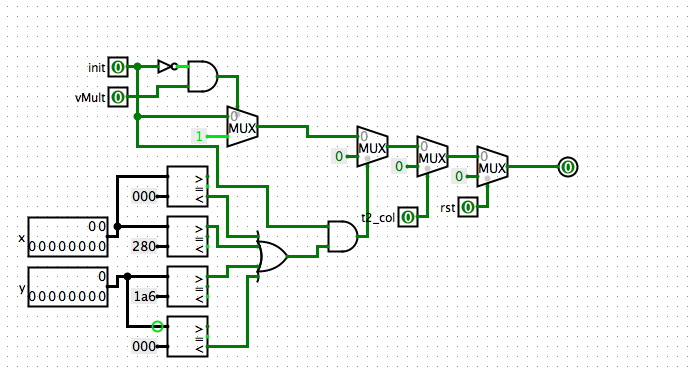
\includegraphics[width=1\textwidth]{init.png} 
		\caption{Init logic module}
	\end{center}
\end{figure}

This module specifies what value init should be. It uses comparators to determine if the x or y location of the projectile is off the screen. If this is the case, or if the reset or collision flags are triggered, init is set to 0. Otherwise, it uses logic from the output of the power module to determine if init should be set to 1. Init should only be set to one if power outputs a non-zero value and init is currently 0.

\begin{figure}[H]
	\begin{center}
		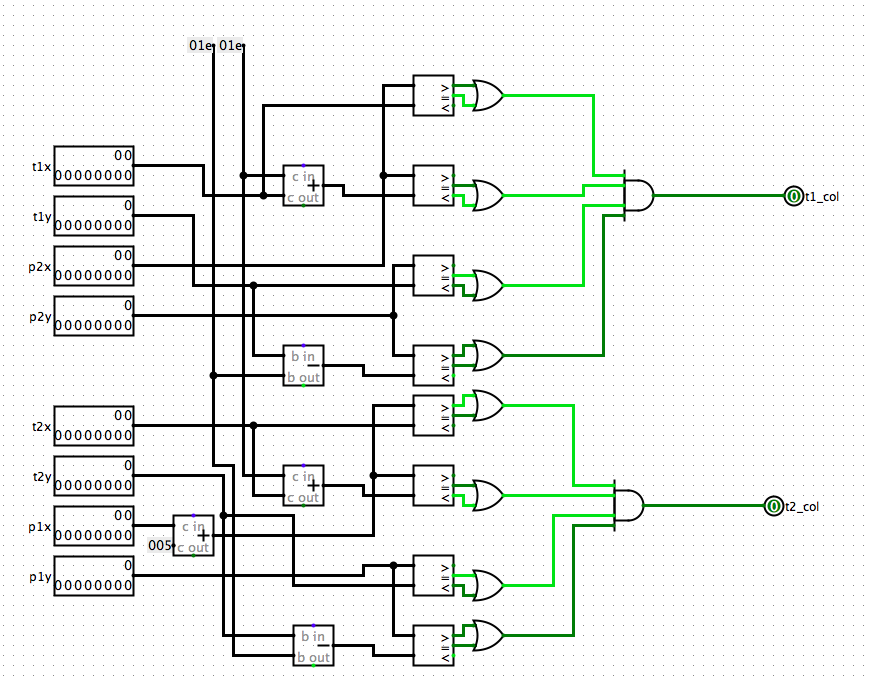
\includegraphics[width=1\textwidth]{coldet.png} 
		\caption{Collision detector module logic}
	\end{center}
\end{figure}

This module checks if either projectile has collided with the other tank. It does this by using comparators to see if the projectile's x and y locations are within the tank's x and y locations. A subtractor is used to check the y range. An adder is used on the projectile traveling right because we need to check if the right side of the projectile collided with the left side of the tank.

\begin{figure}[H]
	\begin{center}
		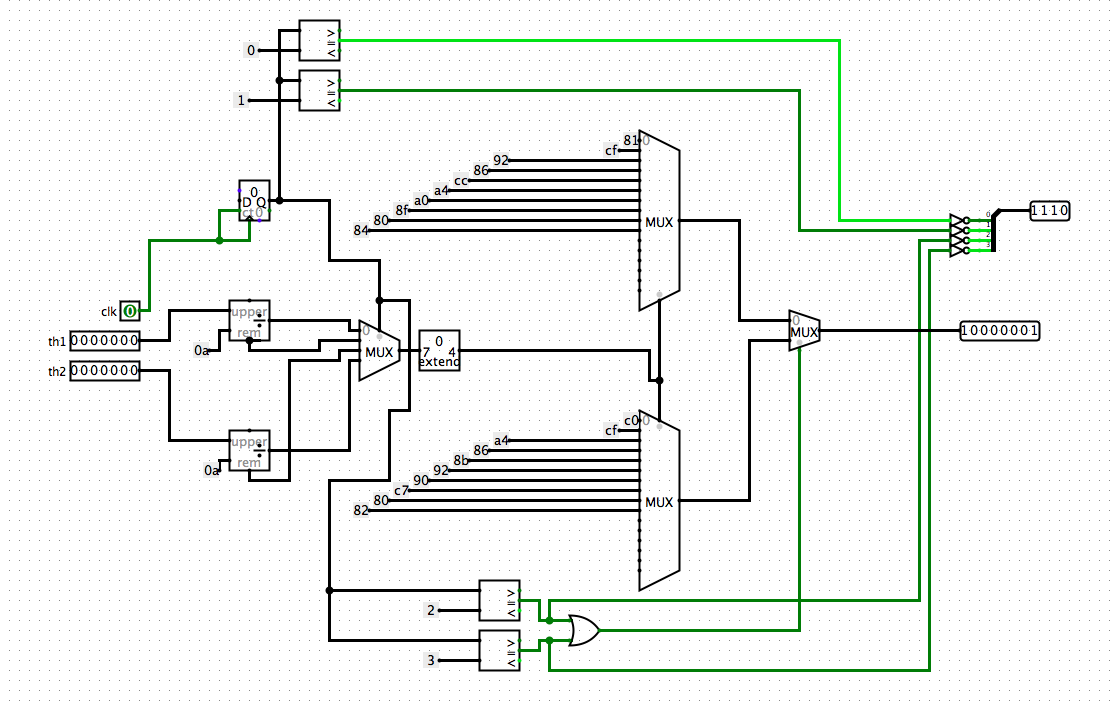
\includegraphics[width=1\textwidth]{sevenseg.png} 
		\caption{Seven segment display module logic}
	\end{center}
\end{figure}

This module displayes tank health on the seven segment display. It takes in a fast clock to switch between the segments quickly. To determine which segment to display the number for, we have a 2 bit counter that overflows back to 0. We used 4 comparators to determine which of the 4 segments should display (if the counter is 0, display the first segment, if the counter is 1, display the second, and so on). Each of the tank healths are passed into a divider. The result represents the tens digit of health, and the remainder represents the ones digit. We pass these values into a MUX, which is selected by whatever segment is displaying from the counter. Then, this number is cast to 4 bits. We can do this because we know the number has to be 0-9. This number is then passed into two MUXes. These MUXes determine what bits should be lit up on the segment. We have two because when playing the game, the two players will be facing different directions, so we flipped the numbers on one side of the seven segment display for easier reading. The results of both of these MUXes are passed into another MUX which determines whether it should used the flipped number or not based on the segment being displayed. The seg and an values are the outputs to the board.

\begin{figure}[H]
	\begin{center}
		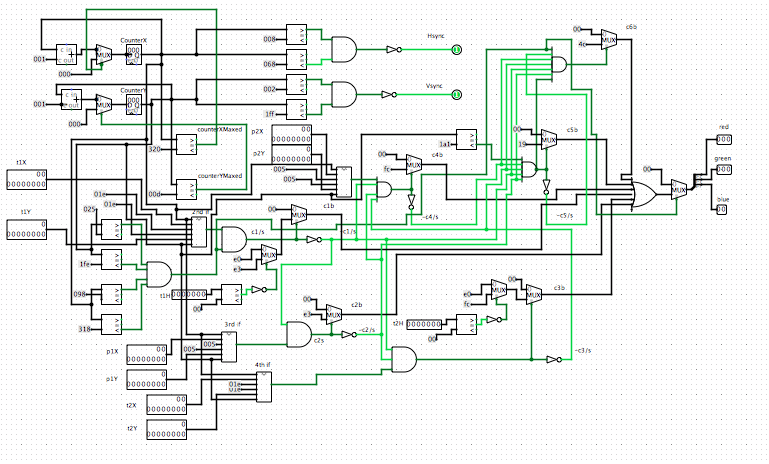
\includegraphics[width=1\textwidth]{vgaOut} 
		\caption{VGA module logic}
	\end{center}
\end{figure}

This vga module takes in the t1X, t1Y, t2X, t2Y, p1X, p1Y, p2X, p2Y, t1H and t2H as input and outputs Hsync, Vsync, red, green and blue. A 25MHz clock is also input and drives the two counter registers that you can see in the top left of the above diagram.  For simplicity's sake, the clock is not included in the image above. The above image is the digital design logic for the VGA controller module.

\begin{figure}[H]
	\begin{center}
		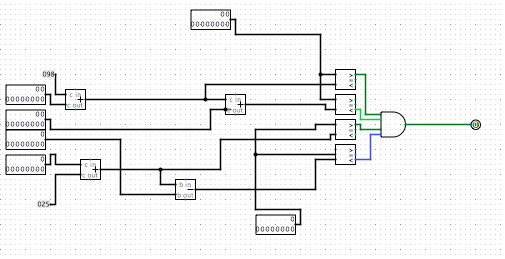
\includegraphics[width=1\textwidth]{vgaBlackBox} 
		\caption{VGA black box 1}
	\end{center}
\end{figure}

The above image is the digital design logic for a black box included in the diagram showing the logic for the VGA controller module.  The circuit in the image above corresponds to the long rectangular module in the VGA diagram.


%----------------------------------------------------------------------------------------
%	SECTION 3
%----------------------------------------------------------------------------------------

\section*{Simulation}

%Simulation documentation (10%). Document all the simulation efforts (what
%requirements are tested and what the test cases are), document bugs found
%during simulation, and provide simulation waveforms. Include all simulation
%testbench code source files.


\section*{Conclusion}


%Conclusion (5%). Summary of the design. Difficulties you encountered, and
%how you dealt with them. General suggestions for improving the lab, if any.

%----------------------------------------------------------------------------------------
%	BIBLIOGRAPHY
%----------------------------------------------------------------------------------------

%\bibliographystyle{apalike}

%\bibliography{sample}

%----------------------------------------------------------------------------------------


\end{document}